\documentclass{article}

%% Denote paragraphs with vertical space rather than indenting (not critical)
\usepackage{parskip}

%% Support for URL in introductory text (not needed for main example)
\usepackage{url}

%% *** Enable TikZ ***
\usepackage{tikz}

%% *** TikZ library ***
\usetikzlibrary{positioning,calc,backgrounds}

\begin{document}

%% Introductory Text
Example 4.4 from the book\\
\emph{Unlocking LaTeX Graphics: A Concise Guide to Ti$k$Z/PGF and PGFPLOTS}.\\
For more information, visit \url{https://latex-graphics.com}.
\par\bigskip

%% *** START OF EXAMPLE CODE ***
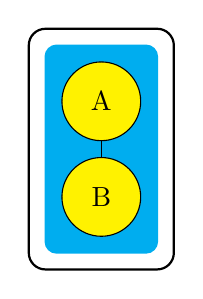
\begin{tikzpicture}[every node/.style={draw, fill=yellow, circle, minimum size=1cm}]
  \path node (A) {A} node[below=2mm of A] (B) {B} edge (A);
  \begin{scope}[on background layer]
    \filldraw[cyan,thick, rounded corners]
      ($(current bounding box.south west)+(-0.2,-0.2)$)
      rectangle
      ($(current bounding box.north east)+(0.2,0.2)$);
  \end{scope}
  \draw[thick, rounded corners=6pt]
    ($(current bounding box.south west)+(-0.2,-0.2)$)
    rectangle ($(current bounding box.north east)+(0.2,0.2)$);
\end{tikzpicture}
%% *** END OF EXAMPLE CODE ***

\end{document}
